\documentclass[]{beamer}
%\usepackage[utopia]{mathdesign}
%\usepackage[no-math]{fontspec}
%\setmainfont{Liberation Serif}

\usepackage{minted}
% \usepackage{redhat}
\usepackage{hyperref}
\usepackage{ccicons}
\usepackage{ulem}

\usepackage{tikz}
\usetikzlibrary{arrows,shapes,snakes,automata,backgrounds,petri}

%gets rid of bottom navigation bars
\setbeamertemplate{footline}[frame number]{}

%gets rid of navigation symbols
\setbeamertemplate{navigation symbols}{}

\newcommand{\done}{\textcolor{teal}{\checkmark}}
\newcommand{\pull}[3]{\href{https://github.com/systemd/#1/pulls/#2}{#3 (\##2)}}
\newcommand{\pulldone}[3]{\pull{#1}{#2}{#3} \done}
\newcommand{\commit}[3]{\href{https://github.com/systemd/#1/commit/#2}{#3 (#2)}}
\newcommand{\commitdone}[3]{\commit{#1}{#2}{#3} \done}
%\newcommand\pp\pause
\newcommand\pp{}


\title{\textsc{Mkosi-initrd (in Fedora)}}
\author{Zbigniew Jędrzejewski-Szmek}
\institute{%
  
\includegraphics[width=0.4\textwidth]{images/Logo-redhat-color-375.png}\\
  \medskip
  \textit{zbyszek@in.waw.pl}\\
  \medskip
  \ccbysa
}
\date{\tiny DevConf Brno 2023, 18.6.2023}

\begin{document}

\setbeamertemplate{itemize items}[square]

\begin{frame}
\titlepage % Print the title page as the first slide
\end{frame}

\begin{frame}
  \frametitle{(instead of) Intro}

  \pp

  see Vitaly Kuzentsov's \\
  \href{https://devconfcz2023.sched.com/event/1MYg7/confidential-vms-in-the-cloud}
       {\textsc{``Confidential VMs in the cloud''}}
  \\\quad
  Christophe de Dinechin's \\
  \href{https://devconfcz2023.sched.com/event/1MYgS/confidential-computing-from-host-to-workload}
       {\textsc{``Confidential Computing, from host to workload''}}
  \\\quad
  \pp

  signed code only
  \\\pp
  => kernel+initrd combined into a UKI (and signed!)
  \\\pp
  => initrd must be built by the vendor/distro
  \\\pp
  => no local modifications
  \\\pp
  => a system designed for local modifications is not useful
  \\\quad
  \\\pp

  if we are building in a package builder, let's build directly from distro packages\\
    (we \textit{could} build from files in the fs, but why?)
\end{frame}

\begin{frame}
  \frametitle{Current approach to initrds}

%%   \pp
%%   goals:

%%   \begin{itemize}
%%   \item speed → event-driven logic
%%   \item speed → size minimization
%%   \item flexibility, versability, end-user choice
%%   \item local configuration embedded in the initrd
%%   \end{itemize}

%%   \pp
%%   results:

  \pp

  \begin{itemize}
  \item local builds take files from host fs,\\
    \texttt{ldd} to resolve dependencies
  \pp

  \item the packaging layer is duplicated
  \pp

  \item lots of CPU cycles burnt during each kernel update
  \pp

  \quad

  \item at runtime: custom logic (e.g. dracut's initqueue)
  \pp

  \item custom tools (e.g. scripts to bring up LVM, dracut modules)
  \pp

  \item different execution environment
  \pp

  \item complexity (in particular when dracut is used with systemd)
  \pp

  \quad

  \item very little sharing of initrd logic between distros
  \end{itemize}
\end{frame}

\begin{frame}
  \frametitle{mkosi}
  \framesubtitle{``\textbf{M}a\textbf{K}e \textbf{O}perating \textbf{S}ystem \textbf{I}mage''}

  Build OS images from distro packages (\texttt{dnf}, \texttt{apt}, \texttt{pacman})
  \pp

  \vfill

  Now uses \texttt{systemd-repart} → (partially) unprivileged operation
  \\

  dnf5
  \\

  Profiles and [Match] sections
  \\

  [mkosi 15, not released yet]
\end{frame}

\begin{frame}
  \frametitle{What is mkosi-initrd?}
  \pp
  Just a few config files for mkosi ;)

  \vfill

  \url{https://github.com/systemd/mkosi-initrd}\vspace{-5em}
\end{frame}

\begin{frame}
  \frametitle{Benefits}

  \begin{itemize}
  \item \textbf{less} things
    \pp
  \item we use package dependency resolution mechanism
    \pp
  \item we let rpm/deb/pacman handle 98\% of the installation
    \pp
  \item we don't pull files from the host
    \pp
  \item images can be reproducible
    \pp
  \item images are the same for everyone
    \pp
  \item images can be easily signed
    \pp
  \item systemd does the heavy lifting in the initrd
%%     \pp
%%   \item bash helpers → compiled programs
%%     \pp
%%   \item developers don't need to learn another system\\
%%     (initrd is like a normal system,\\
%%     \phantom( just on an fs not backed by a disk)
%%     \pp
%%   \item clear ownership of bugs
%%     \pp
%%   \item initrd infrastructure can be shared between distros
  \end{itemize}
\end{frame}

\begin{frame}
  \frametitle{Drawbacks}

  We get fully functional initrds, but…
  \\\quad
  \pp

  The initrds are \textbf{bigger}.\\
  \pp
  Most of the difference is caused by kernel modules
  \\\quad

  \pp
  Only some subset of installations is supported
\end{frame}

\begin{frame}
  \frametitle{Consequences of centralized builds}
  \framesubtitle{If we use pre-built images, how to deliver differentiated code?}
  \pp

  \begin{enumerate}
  \item initrd variants\pp
  \item credentials\pp
  \item systemd-sysexts\pp
  \item systemd-confexts\pp
  \item ``addons''
  \end{enumerate}

%%   \vfill

%%   \pp
%%   Building of sysexts depends build reproducibility of the initrd
\end{frame}

\begin{frame}
  1st extension mechanism: credentials
\end{frame}

\begin{frame}
  \frametitle{Credentials}
  \pp

  A generic mechanism:\\\\
  data → \\
  file (\texttt{/etc/credstore/data}) | other storage → \\
  service has \texttt{LoadCredential=data} → \\
  manager passes the credential → \\
  service sees \texttt{\$CREDENTIALS\_DIRECTORY/data}

  \pp
  \quad

  file | pipe | \\
  qemu \texttt{SMBIOS} | \texttt{fw\_cfg} | \\
  kernel command-line | \\
  boot loader | \\
  inherited credential
\end{frame}

\begin{frame}[fragile]
  \frametitle{Credential encryption}
  \framesubtitle{(with machine keys)}

  \pp
  data → \\
  \textbf{\texttt{systemd-creds encrypt}} → \\
  file | other storage → \\
  \texttt{LoadCredential\textbf{Encrypted}=} → \\
  \textbf{manager decrypts} → \\
  service sees \texttt{\$CREDENTIALS\_DIRECTORY/data}

  \pp
  \quad

  Encryption with:\\
  - \texttt{/var/lib/systemd/credential.secret}
  \\
  - TPM2
  \\
  - both

  \vfill

  \small
  \url{https://systemd.io/CREDENTIALS}
\end{frame}

\begin{frame}
  2nd extension mechanism: confexts
\end{frame}

\begin{frame}
  \frametitle{confexts (and sysexts)}
  \framesubtitle{``Configuration Extensions''\\
                 ``System Extensions''}

  sysext — partial system image that is \texttt{overlayfs}ed on the host system:
  \textcolor{blue}{\texttt{/usr}} and \textcolor{blue}{\texttt{/opt}}
  \\\quad\pp

  confext — partial system image that is \texttt{overlayfs}ed on the host system:
  \textcolor{blue}{\texttt{/etc}}
  \\\quad\pp
\end{frame}

\begin{frame}
  \frametitle{Discoverable Disk Images}

  \href{https://uapi-group.org/specifications/specs/discoverable_partitions_specification/}{The Discoverable Partitions Specification}\\
  (recognition of file system role by part-type UUID)
  \\\quad\pp

  \texttt{systemd-dissect <image>}
  \\\quad\pp

  \texttt{systemd-dissect --mount <image> <path>}
  \\\quad\pp

  \texttt{systemd-dissect --mtree <image>}
\end{frame}

\begin{frame}
  \frametitle{systemd-dissect <image>}

  \hspace*{-2em}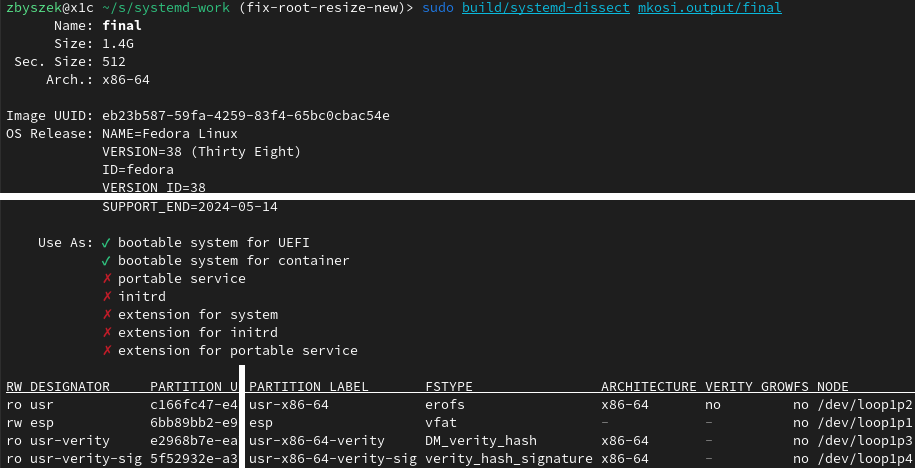
\includegraphics[width=1.15\textwidth]{images/systemd-dissect.png}
\end{frame}

\begin{frame}
  \frametitle{What are DDIs good for?}

  operating system image → hardware or VM or container
  \\\quad

  portable service
  \\\quad

  % initrd?

  system extension
  \\\quad

  initrd extension
  \\\quad

  portable service extension
\end{frame}

%% \begin{frame}
%%   \frametitle{What are System Extensions good for?}

%%   \pp
%%   \textcolor{teal}{Reminder:}{ }\begin{minipage}[t]{0.8\linewidth}
%%     the initrd is a compressed cpio archive

%%     \quad

%%     a sysext is a GPT image with
%%     three partitions:\\
%%     the filesystem (e.g.\ compressed squashfs),
%%     dm-verity for the filesystem,
%%     signature for the verity data
%%   \end{minipage}

%%   \quad

%%   \begin{itemize}
%%     \pp
%%   \item a network configuration daemon + sshd

%%     \pp
%%   \item nfs / RAIDs / clevis / network storage

%%     \pp
%%   \item the full graphical stack\pp: a11y! \pp i18n!

%%     \pp
%%   \item the full sound stack\pp: a11y!

%%     \pp
%%   \item hardware enablement, incl. bluetooth

%%     \pp
%%   \item (suggestions welcome)
%%   \end{itemize}
%% \end{frame}

%% \begin{frame}
%%   \frametitle{What does the kernel say?}

%%   \pp
%%   (the short answer: it doesn't care)

%%   \hfill

%%   \pp
%%   the long answer:
%%   the initrd is just an in-memory file system\\
%%   \texttt{/init} is started instead of \texttt{/sbin/init}
%% \end{frame}

%% \begin{frame}
%%   \frametitle{New goals}

%%   \begin{itemize}
%%     \pp
%%   \item reuse distro packaging
%%     \pp
%%   \item use systemd in the initrd
%%     \pp
%%   \item use normal services
%%     \pp
%%   \item standard userspace environment
%%     \pp
%%   \item reasonable size
%%     \pp

%%   \quad

%%   \item build reproducible initrd images
%%     \pp
%%   \item build initrd images on vendor systems
%%     \pp
%%   \item sign the kernel + initrd
%%     \pp
%%   \item build a set of System Extension images for the initrd
%%     \pp
%%   \item sign those too
%%     \pp

%%   \quad

%%   \item maintainers of user-space packages handle ``initrd bugs''
%%   \end{itemize}
%% \end{frame}

\begin{frame}
  3rd extension mechanism: ``addons''
\end{frame}

\begin{frame}[fragile]
  \frametitle{Unified Kernel Images}
  \vfill

  Lots of tooling-level work for Unified Kernel Images (UKIs)\\
  - ukify: python-pefile, config files, sbsign/pesign, addons, SBAT\\
  - \texttt{systemd-measure} to precalculate PCR measurement after boot\\
  - \texttt{kernel-install/60-ukify.install}\\
    ~~~~~~(\texttt{initrd\_generator=ukify})\\
  - \texttt{kernel-install/90-uki-copy.install}\\
    ~~~~~~(\texttt{layout=uki})\\

  - \texttt{bootctl kernel-identify / kernel-inspect}
\end{frame}

\begin{frame}
  \frametitle{How to deliver differentiated code?}
  \pp

  \begin{enumerate}
  \item initrd variants\pp
  \item credentials → encrypted via TPM\pp
  \item systemd-sysexts → checked via kernel keyring
  \item systemd-confexts\pp
  \item ``addons'' → checked via SecureBoot db / shim
  \end{enumerate}

  \vfill

  \pp
  Building of sysexts depends build reproducibility of the initrd
\end{frame}

\begin{frame}
  \frametitle{Progress over the last few months}

  \begin{itemize}
  \item \texttt{mkosi-initrd} has a growing test suite (booting different storage types)
  \item \texttt{mkosi} supports builds as an unprivileged user
  \item \texttt{systemd} is getting new credential features
  \item \texttt{systemd} has new \texttt{ukify} helper to builds UKIs
  \item Fedora 38 Change for Unified Kernel Images for VMs
  \item New kernel package split in Fedora (\texttt{kernel-modules-core} finally)
  \item GRUB2 might get support for UKIs (\url{https://github.com/osteffenrh/grub2})
  \item Fedora 39 Change for \texttt{mkosi-initrd}
        (\small\url{https://fedoraproject.org/wiki/Changes/mkosi-initrd})
  \end{itemize}
\end{frame}

\begin{frame}[fragile]
  \frametitle{Links}

  \url{https://github.com/systemd/mkosi}

  \url{https://github.com/systemd/mkosi-initrd}

  \url{https://www.freedesktop.org/software/systemd/man/systemd-sysext.html}

  {
    \small
    \url{https://gitlab.com/cryptsetup/cryptsetup/-/wikis/DMVerity}\\
    \color{gray}{\url{https://www.kernel.org/doc/html/latest/admin-guide/device-mapper/verity.html}}
    }

  \url{https://www.kernel.org/doc/html/latest/filesystems/overlayfs.html}

  \quad

  These slides:
  \url{https://github.com/keszybz/mkosi-initrd-talk/raw/main/fosdem2023-buildling-initrds-in-a-new-way.pdf}

  \quad
  \pp

  \hfill \textcolor{red}{QUESTIONS?} \textcolor{green}{\bf /} \textcolor{red}{EOF} \hfill{}

\end{frame}


\begin{frame}
  \frametitle{Objections?}

% If you have some experience in this area,
% and you think that this just infeasible/inefficient/unreasonable, consider that:

  \begin{itemize}
    \pp
    \item
      systemd was already used in the initrd
    \pp
    \item
      the first thing systemd does is to set up the environment
    \pp
    \item
      having tools that support running in a custom environment is hence not useful
    \pp
    \item
      after removing custom logic we don't need to add anything back
    \pp
    \item
      the ecosystem is moving away from scripts towards compiled daemons
    \pp
    \item
      most of the code is in shared libraries, which are installed in full because of link dependencies
    \pp
    \item
      error handling, timeouts, retries, localized messages, event-driven logic, netlink,
      D-bus, all are much easier with ``real'' code
  \end{itemize}
\end{frame}



\end{document}
